\documentclass[a4paper,oneside,brazil,11pt,a4paper,openright,titlepage,
                usenames,dvipsnames]{book}
% Classe alternativa, apropriada para impressão frente-verso.
% \documentclass[11pt,a4paper,openright,titlepage]{book}

\usepackage[utf8]{inputenc}
\usepackage[T1]{fontenc}
\usepackage[brazilian]{babel}
\usepackage{lmodern}
\usepackage{array}
\usepackage{verbatim}
\usepackage{calc}
\usepackage{textcomp}
\usepackage{gensymb}
\usepackage{amsfonts}
\usepackage{amsmath}
\usepackage[thmmarks,amsmath]{ntheorem}%\usepackage{amsthm}
\usepackage{amssymb}
\usepackage{graphicx}
\usepackage{float}
\usepackage[]{subfigure}
\usepackage{epsfig}
\usepackage{boxedminipage}
\usepackage{geometry}
\usepackage{theorem}
\usepackage{fancybox}
\usepackage{fancyhdr}
\usepackage{ifthen}
\usepackage{afterpage}
\usepackage{color}
\usepackage{colortbl}
\usepackage{rotating}
\usepackage{makeidx}
\usepackage{indentfirst}
\usepackage{import}
\usepackage{enumitem}
\usepackage[hyphens]{url}
\usepackage{hyperref}

\usepackage{ft2unb}

\makeindex

\makeatother

\begin{document}
\setcounter{secnumdepth}{4}
\setcounter{tocdepth}{3}
\pagestyle{empty}

\grau{Engenheiro de Controle e Automação}

\tipodemonografia{TRABALHO DE GRADUAÇÃO}

% Título
\titulolinhai{RISC-V SiMPLE:}
\titulolinhaii{Projeto e desenvolvimento de processadores RISC-V}
\titulolinhaiii{com a ISA RV32IMF usando as microarquiteturas}
\titulolinhaiv{ Uniciclo, Multiciclo e Pipeline em FPGA}

% Autores
\autori{Arthur de Matos Beggs}
\autorii{}
\autoriii{}

% Membros da banca
\membrodabancai{Prof.\ Marcus Vinicius Lamar, CIC/UnB}
\membrodabancaifuncao{Orientador}

\membrodabancaii{Prof.\ Ricardo Pezzuol Jacobi, CIC/UnB}
\membrodabancaiifuncao{Examinador Interno}


\membrodabancaiii{Prof.\ Marcelo Grandi Mandelli,CIC/UnB}
\membrodabancaiiifuncao{Examinador Interno}

\membrodabancaiv{}
\membrodabancaivfuncao{}

\membrodabancav{}
\membrodabancavfuncao{}

% Data de defesa
\mes{Maio}
\ano{2021}

% Comandos para criar a capa e a página de assinaturas
\capaprincipal{}
\capaassinaturas{}

% Ficha Catalográfica
\noindent \textbf{FICHA CATALOGRÁFICA}

\noindent %
\fbox{\begin{minipage}[t]{1\columnwidth}%
ARTHUR, DE MATOS BEGGS

RISC-V SiMPLE,

\medskip{}


{[}Distrito Federal{]} 2019.

\medskip{}


$n^{\circ}???$, ???p., 297 mm (FT/UnB, Engenheiro, Controle e Automação, 2019).
Trabalho de Graduação \textendash{} Universidade de Brasília. Faculdade
de Tecnologia.

\medskip{}


1. RISC-V\hfill{}2. ???\hfill{}

\medskip{}


I. Mecatrônica/FT/UnB\hfill{}II. Título (Série)\hfill{}

%
\end{minipage}}

\noindent \medskip{}


\noindent \textbf{REFERÊNCIA BIBLIOGRÁFICA}

BEGGS, ARTHUR DE MATOS, (2019). RISC-V SiMPLE. Trabalho de Graduação
em Engenharia de Controle e Automação, Publicação FT.TG-$n^{\circ}???$,
Faculdade de Tecnologia, Universidade de Brasília, Brasília, DF, ???p.

\noindent \bigskip{}


\noindent \textbf{CESSÃO DE DIREITOS}

\noindent AUTOR: Arthur de Matos Beggs

TÍTULO DO TRABALHO DE GRADUAÇÃO: RISC-V SiMPLE.

\noindent \medskip{}


\noindent GRAU: Engenheiro\hfill{}ANO: 2019\hfill{}

\noindent \medskip{}


É concedida à Universidade de Brasília permissão para reproduzir cópias
deste Trabalho de Graduação e para emprestar ou vender tais cópias
somente para propósitos acadêmicos e científicos. O autor reserva
outros direitos de publicação e nenhuma parte desse Trabalho de Graduação
pode ser reproduzida sem autorização por escrito do autor.

\noindent \bigskip{}


\noindent \rule[0.5ex]{1\columnwidth}{1pt}

\noindent Arthur de Matos Beggs

\noindent SHCGN 703 Bl G Nº 120, Asa Norte

\noindent 70730-707 Brasília \textendash{} DF \textendash{} Brasil.


% Dedicatória
\frontmatter

\dedicatoriaautori{}
\dedicatoriaautorii{}
\dedicatoriaautoriii{}
\dedicatoria{}

% Agradecimentos
\agradecimentosautori{}
\agradecimentosautorii{}
\agradecimentosautoriii{}
\agradecimentos{}

\resumo{resumo}{
{
    Desenvolvimento e documentação de uma plataforma de ensino de arquitetura
    de computadores em \textit{Verilog} sintetizável em \textit{FPGA}, com foco
    em um processador com arquitetura do conjunto de instruções \textit{RISC-V}
    implementado em três microarquiteturas para ser utilizado como recurso de
    laboratório na disciplina de Organização e Arquitetura de Computadores da
    Universidade de Brasília.
    A plataforma funciona nas \textit{FPGAs terasIC DE1-SoC} disponíveis no
    laboratório da Universidade, possui periféricos de depuração como
    \textit{display} dos registradores do processador na saída de vídeo, além
    de outros periféricos como \textit{drivers} de áudio e vídeo para uma
    experiência mais completa de desenvolvimento, e permite que o processador
    seja substituído por implementações de diversas arquiteturas de
    \textit{32 bits} com certa facilidade.
}

\medskip{}

Palavras Chave: RISC-V, Verilog, FPGA
}\vspace*{2cm}


\resumo{Abstract}{
{
}

\medskip{}

Keywords: RISC-V, Verilog, FPGA
}

% Listas de conteúdo, figuras e tabelas
\sumario{}
\listadefiguras{}
\listadetabelas{}

% Lista de Símbolos
%TCIDATA{LaTeXparent=0,0,these.tex}


%\chapter*{\setfontarial\mdseries LISTA DE SÍMBOLOS} % se usar ft1unb.sty, descomente esta linha



\chapter*{LISTA DE SÍMBOLOS}

% se usar ft2unb.sty, descomente esta linha



% \subsection*{Símbolos Latinos}

% \begin{tabular}{p{0.1\textwidth}p{0.63\textwidth}>{\PreserveBacklash\raggedleft}p{0.15\textwidth}}
% $v$  & Velocidade linear  & {[}m/s{]}\tabularnewline
% \end{tabular}


% \subsection*{Símbolos Gregos}

% \begin{tabular}{p{0.1\textwidth}p{0.63\textwidth}>{\PreserveBacklash\raggedleft}p{0.15\textwidth}}
% $\omega$ & Velocidade angular & {[}rad/s{]}\tabularnewline
% \end{tabular}


% \subsection*{Grupos Adimensionais}
%
% \begin{tabular}{p{0.1\textwidth}p{0.8\textwidth}}
% i, k & Contador\tabularnewline
% \end{tabular}


% \subsection*{Subscritos}

% \begin{tabular}{p{0.1\textwidth}p{0.8\textwidth}}
% $ref$  & referência \tabularnewline
% $fer$  & ferramenta \tabularnewline
% $sis$  & sistema \tabularnewline
% $des$  & desejado\tabularnewline
% \end{tabular}


% \subsection*{Sobrescritos}

% \begin{tabular}{p{0.1\textwidth}p{0.8\textwidth}}
% $\cdot$  & Variação temporal \tabularnewline
% $-$  & Valor médio \tabularnewline
% \end{tabular}


\subsection*{Siglas}

\begin{tabular}{p{0.1\textwidth}p{0.8\textwidth}}
    {BSD} & {Distribuição de Software de Berkeley --- \textit{Berkeley Software Distribution}}\tabularnewline{}
    {CSR} & {Registradores de Controle e Estado --- \textit{Control and Status Registers}} \tabularnewline{}
    {FPGA} & {Arranjo de Portas Programáveis em Campo --- \textit{Field Programmable Gate Array}} \tabularnewline{}
    {hart} & {\textit{hardware thread}} \tabularnewline{}
    {ISA} & {Arquitetura do Conjunto de Instruções --- \textit{Instruction Set Architecture}} \tabularnewline{}
    {MIPS} & {Microprocessador sem Estágios Intertravados de \textit{Pipeline} --- \textit{Microprocessor without Interlocked Pipeline Stages}} \tabularnewline{}
    {OAC} & {Organização e Arquitetura de Computadores} \tabularnewline{}
    {RISC} & {Computador com Conjunto de Instruções Reduzido --- \textit{Reduced Instruction Set Computer}} \tabularnewline{}
    {SiMPLE} & {Ambiente de Aprendizado Uniciclo, Multiciclo e \textit{Pipeline} --- \textit{Single-cycle Multicycle Pipeline Learning Environment}} \tabularnewline{}
    {RAS} & {Pilha de Endereços de Retorno --- \textit{Return Address Stack}} \tabularnewline{}
    {TTL} & {Lógica Transistor-Transistor --- \textit{Transistor-Transistor Logic}} \tabularnewline{}
     % &  \tabularnewline
     % &  \tabularnewline
\end{tabular}


% Corpo Principal
\mainmatter{}
\setcounter{page}{1}
\pagenumbering{arabic}
\pagestyle{plain}

%% Template de imagem
% \begin{figure}[H]
% \centering
% \includegraphics[width=.7\linewidth]
%     {../images/}
%     \caption[]
%         {}\label{fig:}
% \end{figure}

\chapter{Introdução}\label{cap_intro}
% TODO: Adicionar demanda da plataforma p/ várias FPGAs

%\resumodocapitulo{Resumo opcional}

\section{Motivação}
{
    O mercado de trabalho está a cada dia mais exigente, sempre buscando
    profissionais que conheçam as melhores e mais recentes ferramentas
    disponíveis. Além disso, muitos universitários se sentem desestimulados
    ao estudarem assuntos desatualizados e com baixa possibilidade de
    aproveitamento do conteúdo no mercado de trabalho. Isso alimenta o
    desinteresse pelos temas abordados e, em muitos casos, leva à evasão
    escolar. Assim, é importante renovar as matérias com novas tecnologias
    e tendências de mercado sempre que possível, a fim de instigar o
    interesse dos discentes e formar profissionais mais capacitados e
    preparados para as demandas da atualidade.
}

{
    Hoje, a disciplina de Organização e Arquitetura de Computadores da
    Universidade de Brasília é ministrada utilizando a arquitetura
    \textit{MIPS32}. Apesar da arquitetura \textit{MIPS32} ainda ter
    grande força no meio acadêmico (em boa parte devido a sua simplicidade
    e extensa bibliografia), sua aplicação na indústria tem diminuído
    consideravelmente na última década.
}

{
    Embora a curva de aprendizagem de linguagens \textit{Assembly} de
    alguns processadores \textit{RISC} seja relativamente baixa para quem
    já  conhece o \textit{Assembly MIPS32}, aprender uma arquitetura atual
    traz o benefício de conhecer o \textit{estado da arte} da organização e
    arquitetura de computadores.
}

{
    Para a proposta de modernização da disciplina, foi escolhida a
    \textit{ISA RISC-V} desenvolvida na Divisão de Ciência da Computação da
    Universidade da Califórnia, Berkeley como substituta à
    \textit{ISA MIPS32}.
}


\section{Por que RISC-V?}
{
    A \textit{ISA RISC-V} (lê-se \textit{``risk-five''}) é uma arquitetura
    \textit{open source} com licença \textit{BSD}, o que permite o seu
    livre uso para quaisquer fins, sem distinção de se o trabalho possui
    código-fonte aberto ou proprietário. Tal característica possibilita que
    grandes fabricantes utilizem a arquitetura para criar seus produtos,
    mantendo a proteção de propriedade intelectual sobre seus métodos de
    implementação e quaisquer subconjuntos de instruções
    não-\textit{standard} que as empresas venham a produzir, o que
    estimula investimentos em pesquisa e desenvolvimento.
}

{
    Empresas como Google, IBM, AMD, Nvidia, Hewlett Packard, Microsoft,
    Qualcomm e Western Digital são algumas das fundadoras e investidoras
    da \textit{RISC-V Foundation}, órgão responsável pela governança da
    arquitetura. Isso demonstra o interesse das gigantes do mercado no
    sucesso e disseminação da arquitetura.
}

{
    A licença também permite que qualquer indivíduo produza, distribua e
    até mesmo comercialize sua própria implementação da arquitetura sem ter
    que arcar com \textit{royalties}, sendo ideal para pesquisas
    acadêmicas, \textit{startups} e até mesmo \textit{hobbyistas}.
}

{
    O conjunto de instruções foi desenvolvido tendo em mente seu uso em
    diversas escalas: sistemas embarcados, \textit{smartphones},
    computadores pessoais, servidores e supercomputadores, o que permitirá
    maior reuso de \textit{software} e maior integração de
    \textit{hardware}.
}

{
    Outro fator que estimula o uso do \textit{RISC-V} é a modernização dos
    livros didáticos. A nova versão do livro utilizado em OAC, Organização
    e Projeto de Computadores, de David Patterson e John Hennessy, utiliza
    a \textit{ISA RISC-V}.
}

{
    Além disso, com a promessa de se tornar uma das arquiteturas mais
    utilizadas nos próximos anos, utilizar o \textit{RISC-V} como
    arquitetura da disciplina de OAC se mostra a escolha ideal no momento.
}

\section{O Projeto RISC-V SiMPLE}
{
    O projeto \textit{RISC-V SiMPLE (Single-cycle Multicycle Pipeline
    Learning Environment)} consiste no desenvolvimento de um processador
    com conjunto de instruções \textit{RISC-V}, sintetizável em
    \textit{FPGA} e com \textit{hardware} descrito em \textit{Verilog}. A
    microarquitetura implementada nesse trabalho é uniciclo, escalar, em
    ordem, com um único \textit{hart} e com caminho de dados de 64 bits.
    Trabalhos futuros poderão utilizar a estrutura altamente configurável
    e modularizada do projeto para desenvolver as versões em
    microarquiteturas multiciclo e \textit{pipeline}.
}

{
    O processador contém o conjunto de instruções I (para operações com
    inteiros, sendo o único módulo com implementação mandatória pela
    arquitetura) e as extensões \textit{standard} M (para multiplicação e
    divisão de inteiros) e F (para ponto flutuante com precisão simples
    conforme o padrão IEEE 754 com revisão de 2008). O projeto não
    implementa as extensões D (ponto flutuante de precisão dupla) e A
    (operações atômicas de sincronização), e com isso o \textit{soft core}
    desenvolvido não pode ser definido como de propósito geral, G (que deve
    conter os módulos I, M, A, F e D). Assim, pela nomenclatura da
    arquitetura, o processador desenvolvido é um \textit{RV64IMF}.
}

{
    O projeto contempla \textit{traps}, interrupções, exceções,
    \textit{CSRs}, chamadas de sistema e outras funcionalidades de nível
    privilegiado da arquitetura.
}

{
    O \textit{soft core} possui barramento Avalon para se comunicar com os
    periféricos das plataformas de desenvolvimento. O projeto foi
    desenvolvido utilizando a placa DE2--115 com \textit{FPGA Altera
    Cyclone} e permite a fácil adaptação para outras placas da Altera.
}


\chapter{Revisão Teórica}\label{cap_revisao}

\section{Arquitetura de Computadores}
{}

    \subsection{\textit{MIPS}}
    {}

    \subsection{\textit{RISC-V}}
    {}

\section{Microarquiteturas}
{}

    \subsection{Uniciclo}
    {}

    \subsection{Multiciclo}
    {}

    \subsection{\textit{Pipeline}}
    {}

\section{Representação de \textit{Hardware}}
{}

    \subsection{\textit{Verilog HDL}}
    {}

\section{Síntese Lógica}
{}

    \subsection{Análise e Síntese}
    {}

    \subsection{\textit{Fitting}}
    {}

    \subsection{\textit{Timing Analyzer}}
    {}

\section{Simulação}
{}

\section{Utilizando \textit{Hardware} Real}
{}

    \subsection{\textit{Field Programmable Gate Arrays}}
    {}



\chapter{Sistema Proposto}\label{cap_proposta}

{ O sistema proposto consiste em um \textit{soft-core} da \textit{ISA RISC-V}
    de 32 \textit{bits} com as extensões \textbf{I}, \textbf{M} e \textbf{F},
    podendo ser sintetizado nas versões \textit{RV32I}, \textit{RV32IM} ou
    \textit{RV32IMF}. A extensão \textit{Zicsr} com os Registradores de Controle
    e Estado (\textit{CSR}) é parcialmente implementada em todas as três
    configurações.
}

{ Cada uma das combinações da \textit{ISA} pode ser realizada em três
    microarquiteturas diferentes: unicicilo, multiciclo ou \textit{pipeline} de
    cinco estágios. Assim, o processador pode ser sintetizado em nove
    combinações diferentes.
}

{ O projeto utiliza a placa de desenvolvimento \textit{terasIC DE1-SoC} contendo
    diversos periféricos e um \textit{SoC Intel Altera Cyclone-V}. Vários dos
    periféricos presentes na plataforma tem controladores implementados com
    Entradas e Saídas Mapeadas em Memória (\textit{MMIO}) para que o
    \textit{soft-core} possa utilizá-los. A síntese dos controladores desses
    periféricos, como a saída de vídeo, entrada de teclado e barramento
    \textit{RS-232} é opcional.
}

{ O trabalho também é organizado de forma a facilitar a migração para placas de
    desenvolvimento diferentes da \textit{DE1-SoC} ou trocar o \textit{soft-core}
    desenvolvido por outra implementação, independente da sua \textit{ISA}.
    Todas as opções de configuração estão presentes em um único arquivo,
    centralizando as opções de customização do sistema gerado.
}


\section{Implementação da Microarquitetura Uniciclo}

    \begin{figure}[H]
    \centering
        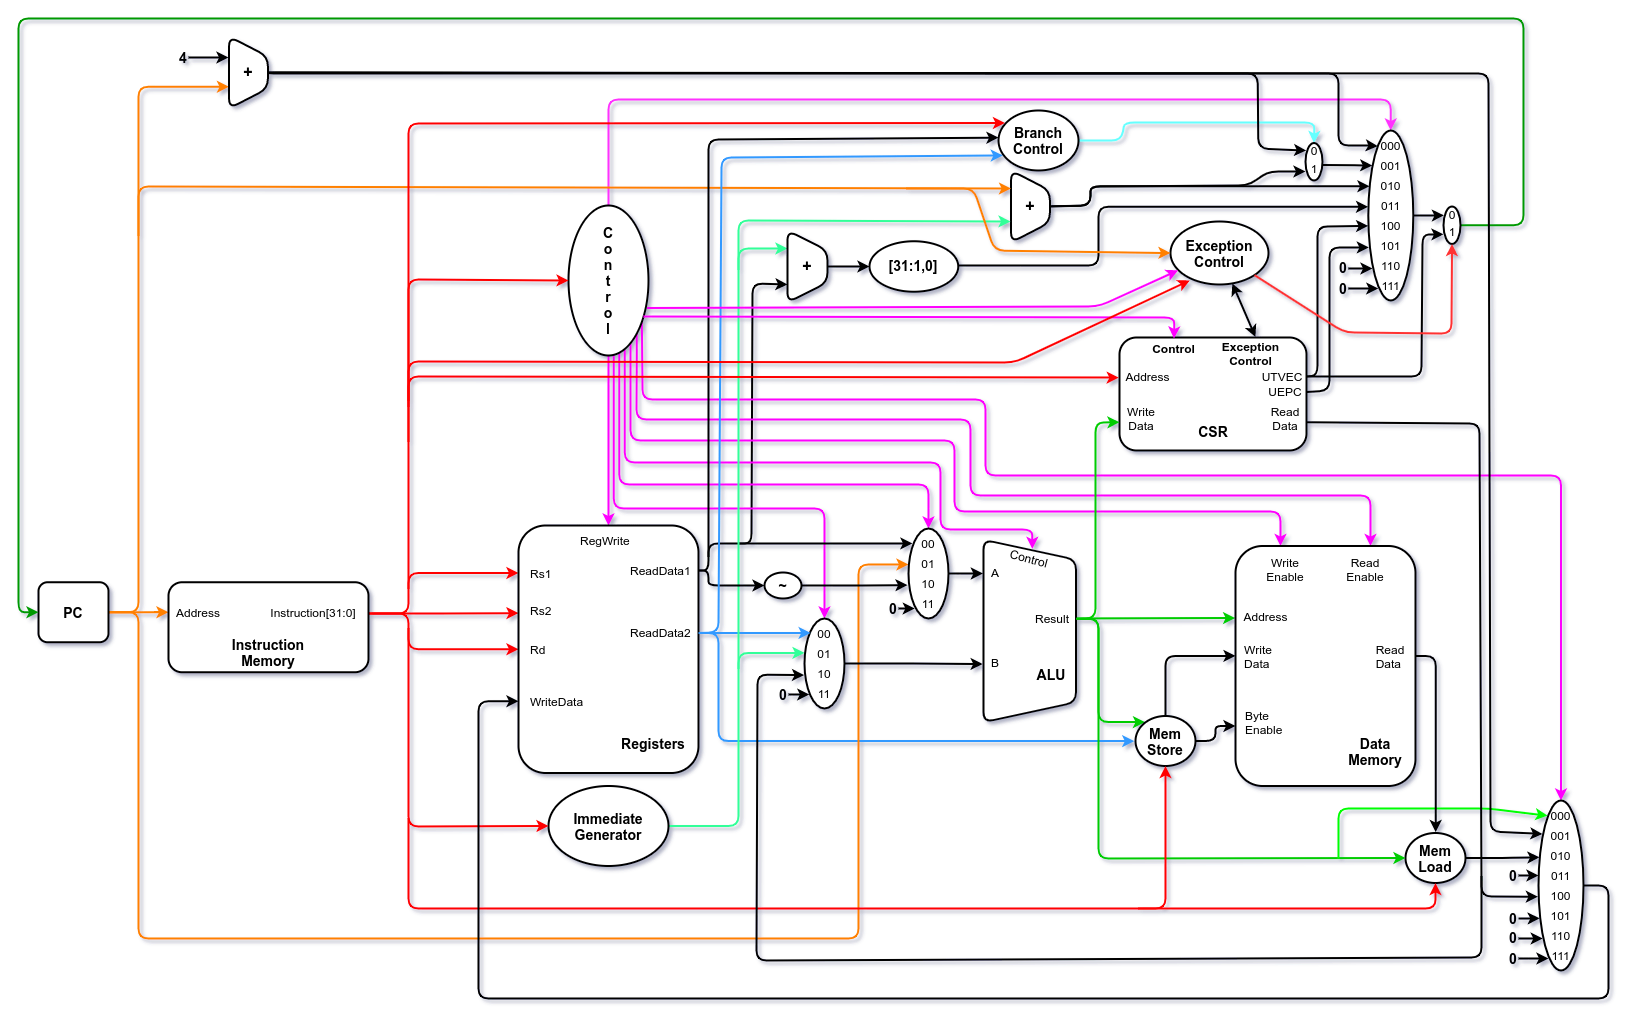
\includegraphics[width=1\linewidth]{../images/uarch_diagrams/singlecycle-RV32I-RV32IM.png}
        \caption{Diagrama da implementação das \textit{ISAs} RV32I e RV32IM na
        microarquitetura uniciclo.}\label{fig:diagram_rv32i_uni}
    \end{figure}

    \begin{figure}[H]
    \centering
        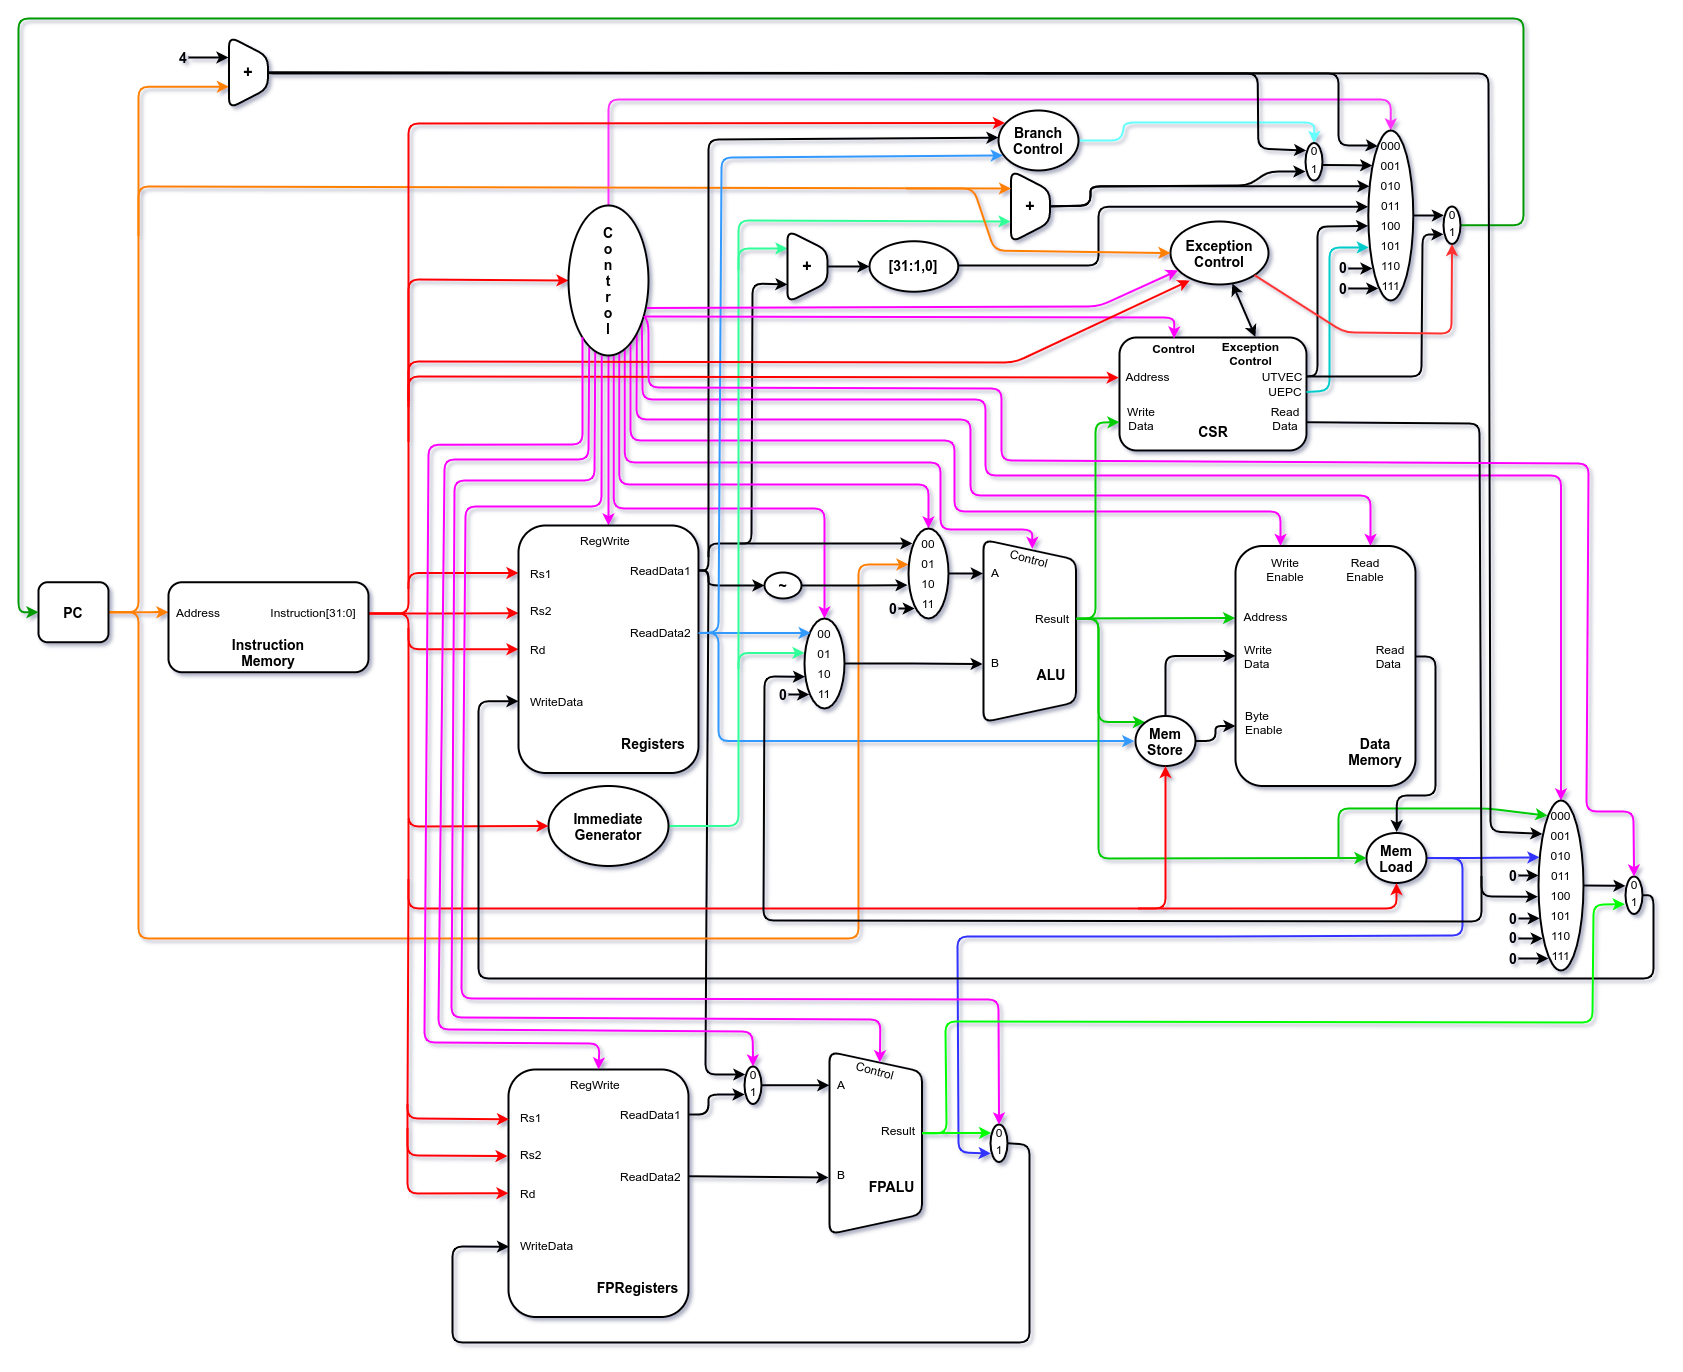
\includegraphics[width=1\linewidth]{../images/uarch_diagrams/singlecycle-RV32IMF.png}
        \caption{Diagrama da implementação da \textit{ISA} RV32IMF na
        microarquitetura uniciclo.}\label{fig:diagram_rv32imf_uni}
    \end{figure}

\section{Implementação da Microarquitetura Multiciclo}

    \begin{figure}[H]
    \centering
        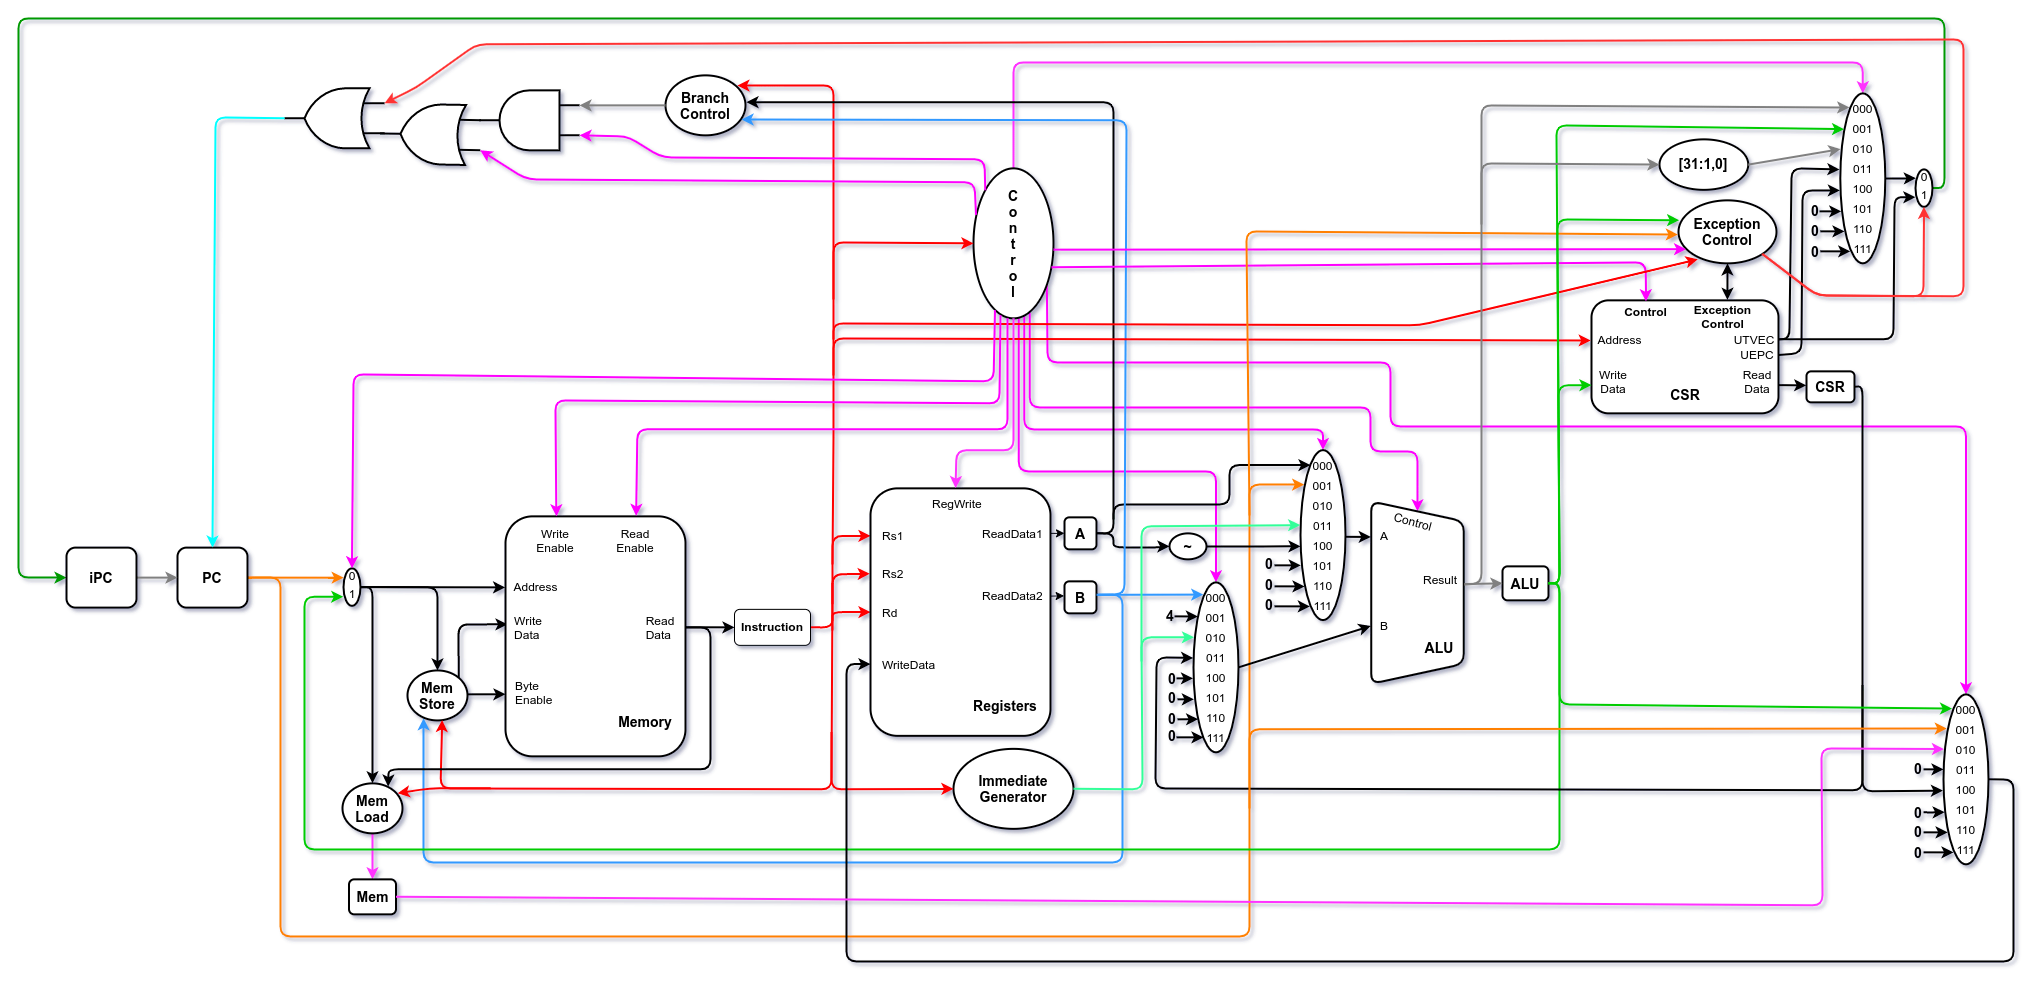
\includegraphics[width=1\linewidth]{../images/uarch_diagrams/multicycle-RV32I-RV32IM.png}
        \caption{Diagrama da implementação das \textit{ISAs} RV32I e RV32IM na
        microarquitetura multiciclo.}\label{fig:diagram_rv32i_multi}
    \end{figure}

    \begin{figure}[H]
    \centering
        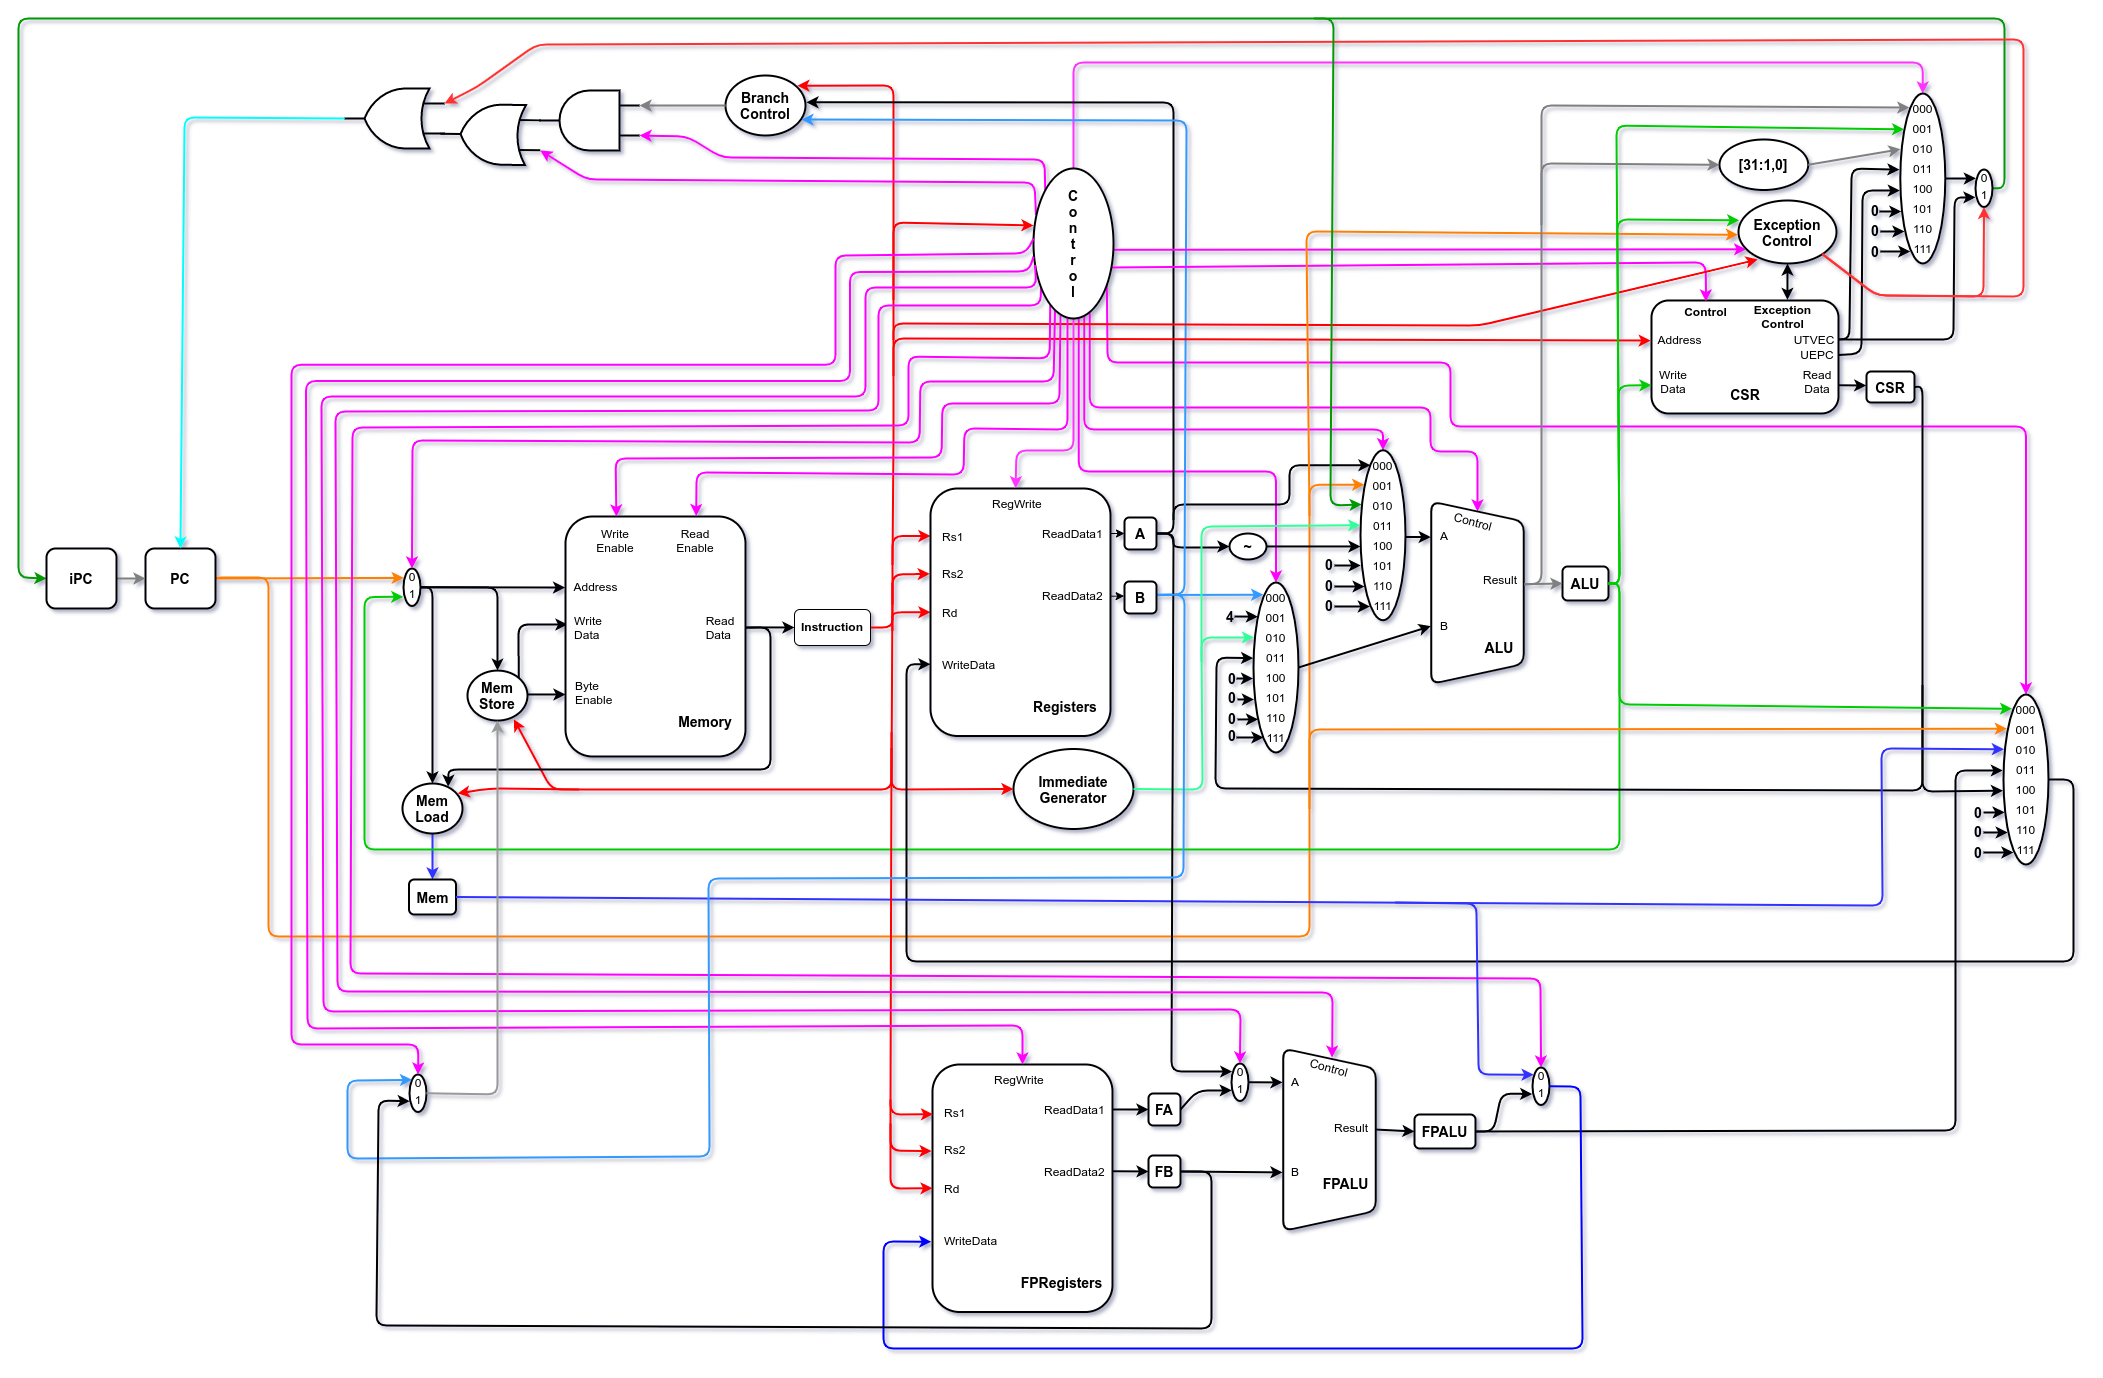
\includegraphics[width=1\linewidth]{../images/uarch_diagrams/multicycle-RV32IMF.png}
        \caption{Diagrama da implementação da \textit{ISA} RV32IMF na
        microarquitetura multiciclo.}\label{fig:diagram_rv32imf_multi}
    \end{figure}


\section{Implementação da Microarquitetura \textit{Pipeline} de 5 Estágios}

    \begin{figure}[H]
    \centering
        
\includegraphics[width=1\linewidth]{../images/placeholder.jpg}
        \caption{Diagrama da implementação das \textit{ISAs} RV32I e RV32IM na
        microarquitetura \textit{pipeline} de 5 estágios.}\label{fig:diagram_rv32i_pipe}
    \end{figure}

    \begin{figure}[H]
    \centering
        
\includegraphics[width=1\linewidth]{../images/placeholder.jpg}
        \caption{Diagrama da implementação da \textit{ISA} RV32IMF na
        microarquitetura \textit{pipeline} de 5 estágios.}\label{fig:diagram_rv32imf_pipe}
    \end{figure}






% \chapter{A Arquitetura RISC-V}\label{cap_arquitetura}

\section{Visão Geral da Arquitetura}
{
    A \textit{ISA RISC-V} é uma arquitetura modular, sendo o módulo base de
    operações com inteiros mandatório em qualquer implementação. Os demais
    módulos são extensões de uso opcional. A arquitetura não suporta
    \textit{branch delay slots} e aceita instruções de tamanho variável. A
    codificação das instruções de tamanho variável é mostrada na
    Figura~\ref{fig:riscv_var_length}. As instruções presentes no módulo
    base correspondem ao mínimo necessário para emular por
    \textit{software} as demais extensões (com exceção das operações
    atômicas).
}

\begin{figure}[H]
\centering
    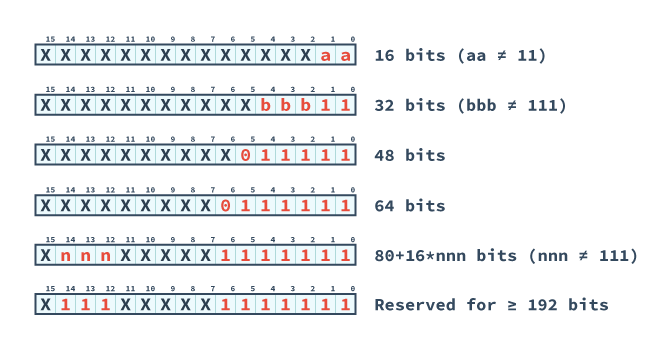
\includegraphics[width=1\linewidth]{../images/RV_InstructionLength.png}
    \caption{Codificação de instruções de tamanho variável da arquitetura
                \textit{RISC-V}}\label{fig:riscv_var_length}
\end{figure}

\clearpage

{
    A nomenclatura do conjunto de instruções implementado segue a
    seguinte estrutura:
}

\begin{itemize}[leftmargin=20mm]
    \item {As letras ``RV'';}
    \item {A largura dos registradores do módulo Inteiro;}
    \item {A letra ``I'' representando a base Inteira. Caso o subconjunto
            Embarcado (\textit{Embedded}) seja implementado, substitui-se
            pela letra ``E'';}
    \item {Demais letras identificadoras de módulos opcionais.}
\end{itemize}

{
    Assim, uma implementação com registradores de 64 bits somente com o
    módulo base de Inteiros é denominado ``RV64I''.
}


\section{Módulo Inteiro}
{}


\section{Extensões}
    \subsection{Extensão M}
    {}


    \subsection{Extensão A}
    {}


    \subsection{Extensão F}
    {}


    \subsection{Extensão D}
    {}


    \subsection{Outras Extensões}
    {}

\section{Arquitetura Privilegiada}
{}


\section{Formatos de Instruções}
{}

\begin{figure}[H]
\centering
    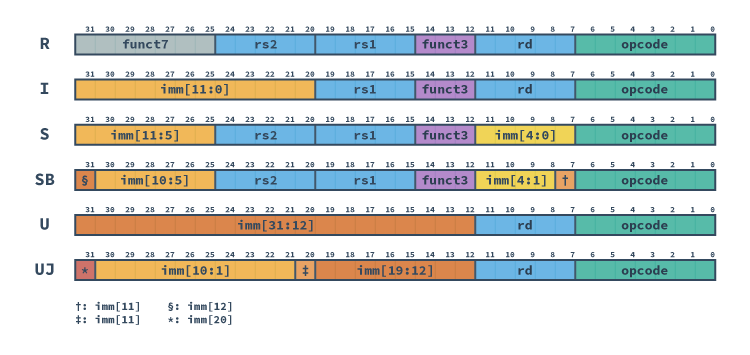
\includegraphics[width=1\linewidth]{../images/RV_Formats.png}
    \caption{Formatos de Instruções da\textit{ISA RISC-V}
        }\label{fig:riscv_formats}
\end{figure}


% \begin{figure}[H]
% \centering
%     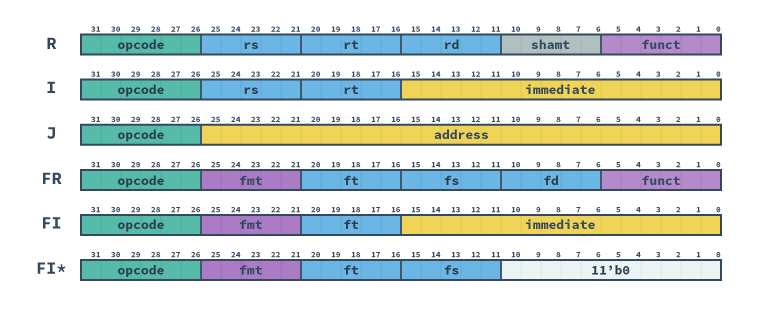
\includegraphics[width=1\linewidth]{../images/MIPS_Formats.png}
%     \caption{Formatos de Instruções da \textit{ISA MIPS32}
%         }\label{fig:mips_formats}
% \end{figure}


\section{Formatos de Imediatos}

\begin{figure}[H]
\centering
    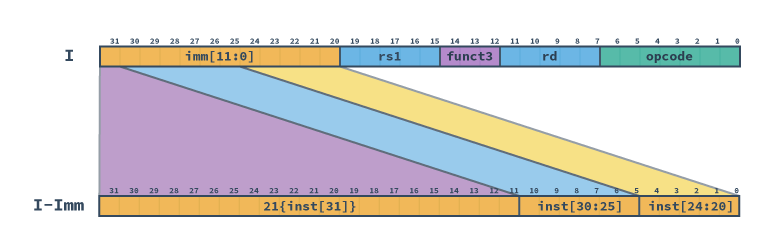
\includegraphics[width=1\linewidth]{../images/RV_I_Imm.png}
    \caption{Formação do Imediato de tipo I
        }\label{fig:riscv_i_imm}
\end{figure}

\begin{figure}[H]
\centering
    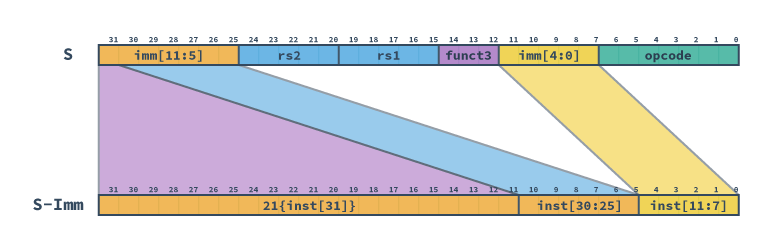
\includegraphics[width=1\linewidth]{../images/RV_S_Imm.png}
    \caption{Formação do Imediato de tipo S
        }\label{fig:riscv_s_imm}
\end{figure}

\begin{figure}[H]
\centering
    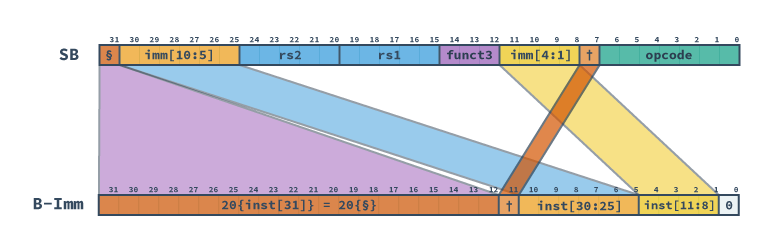
\includegraphics[width=1\linewidth]{../images/RV_B_Imm.png}
    \caption{Formação do Imediato de tipo B
        }\label{fig:riscv_b_imm}
\end{figure}

\begin{figure}[H]
\centering
    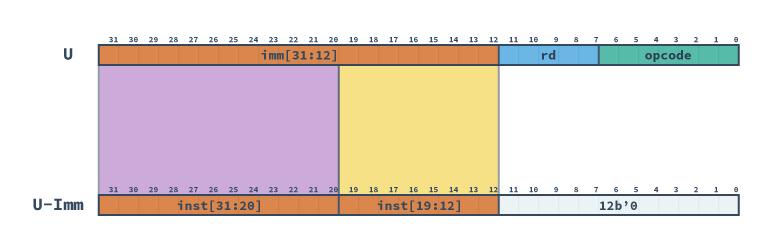
\includegraphics[width=1\linewidth]{../images/RV_U_Imm.png}
    \caption{Formação do Imediato de tipo U
        }\label{fig:riscv_u_imm}
\end{figure}

\begin{figure}[H]
\centering
    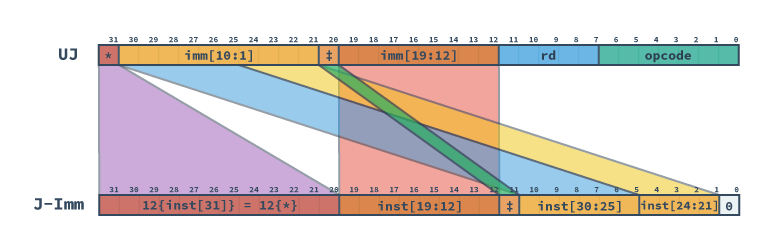
\includegraphics[width=1\linewidth]{../images/RV_J_Imm.png}
    \caption{Formação do Imediato de tipo J
        }\label{fig:riscv_j_imm}
\end{figure}


% \begin{figure}[H]
% \centering
%     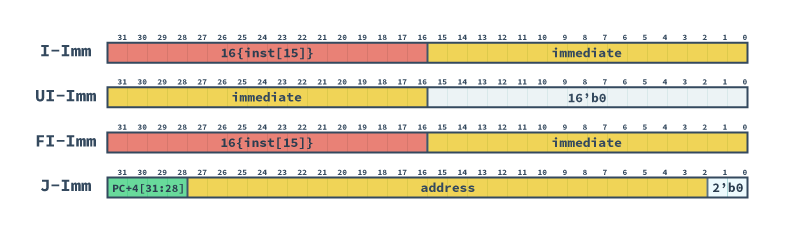
\includegraphics[width=1\linewidth]{../images/MIPS_Immediates.png}
%     \caption{Formatos de Imediato da \textit{ISA MIPS32}}\label{fig:mips_immediates}
% \end{figure}


% \chapter{Field Programmable Gate Arrays}\label{cap_fpga}

{
    \textit{Field Programmable Gate Arrays}---ou \textit{FPGAs}---são circuitos
    integrados que permitem o desenvolvimento de circuitos lógicos
    reconfiguráveis. Por serem reprogramáveis, as \textit{FPGAs} geram uma
    grande economia em tempo de desenvolvimento e em custos como os de
    prototipagem, validação e manufatura do projeto em relação aos circuitos de
    aplicações específicas, os \textit{ASICs}. As \textit{FPGAs} podem ser
    tanto o passo intermediário no projeto de um \textit{ASIC} quanto o meio
    final do projeto quando a reconfigurabilidade e os preços muito mais
    acessíveis forem fatores importantes.
}

{
    Cada fabricante de \textit{FPGAs} possui seus \textit{softwares} de
    desenvolvimento, ou \textit{SDKs}. A indústria de \textit{hardware} é
    extremamente protecionista com sua propriedade intelectual, sendo a maioria
    dessas ferramentas de código proprietário. Para a Intel Altera®, essa
    plataforma é o Quartus Prime®.
}

{
    \textit{FPGAs} mais modernas possuem, além do arranjo de portas lógicas,
    blocos de memória, \textit{PLLs}, \textit{DSPs} e \textit{SoCs}. Os blocos
    de memória internos funcionam como a memória \textit{cache} de um
    microprocessador, armazenando os dados próximo ao seu local de
    processamento para diminuir a latência. Os \textit{PLLs} permitem criar
    sinais de \textit{clock} com diversas frequências a partir de um relógio de
    referência, e podem ser reconfigurados a tempo de execução. \textit{DSPs}
    são responsáveis pelo processamento de sinais analógicos discretizados, e
    podem ser utilizados como multiplicadores de baixa latência. Já os
    \textit{SoCs} são microprocessadores como os ARM® presentes
    em celulares, e são capazes de executar sistemas operacionais como o Linux.
}

{
    Além de disponíveis na forma de \textit{chips} para a integração com placas
    de circuito impresso customizadas, as \textit{FPGAs} possuem \textit{kits}
    de desenvolvimento com diversos periféricos para auxiliar no processo de
    criação de soluções. Esses \textit{kits} são a principal ferramenta de
    aprendizagem no universo dos circuitos reconfiguráveis. No Laboratório de
    Informática da UnB, as placas \textit{terasIC DE1-SoC} com a \textit{FPGA
    Intel® Cyclone V SoC} estão disponíveis para os alunos de OAC desenvolverem
    seus projetos.
}

\clearpage

\section{Arquitetura Generalizada de uma FPGA}
{
    De forma genérica, uma \textit{FPGA} possui blocos lógicos, chaves de
    interconexão, blocos de conexão direta e portas de entrada e saída,
    conforme apresentado na Figura~\ref{fig:fpga_general_arch}.
}

\begin{figure}[H]
\centering
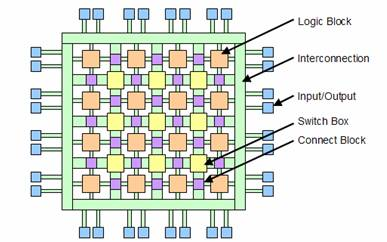
\includegraphics[width=.7\linewidth]
    {../images/fpga_architecture_abstraction_-_olin_college.jpg}
    \caption[Abstração da arquitetura de uma FPGA]
        {Abstração da arquitetura de uma FPGA \quad Fonte: Olin College of
            Engineering}\label{fig:fpga_general_arch}
\end{figure}

{
    Os blocos lógicos possuem \textit{lookup tables}, registradores, somadores
    e multiplexadores. É neles que a lógica reconfigurável é implementada.
}

{
    Já as chaves de interconexão são responsáveis por conectar os diversos
    blocos da \textit{FPGA}. A Figura~\ref{fig:fpga_switch_box} exemplifica
    como é feito o roteamento da malha de interconexão. Os blocos de conexão
    direta são um tipo especial de chave de interconexão, e sua função é ligar
    blocos lógicos adjacentes.
}

{
    Por fim, as portas de entrada e saída conectam a \textit{FPGA} ao ``mundo
    externo'' e.g. \textit{drivers} de áudio e vídeo.
}

\begin{figure}[H]
\centering
\includesvg[width=.5\linewidth]
    {../images/switch_box_wikimedia.svg}
    \caption[Funcionamento da chave de interconexão]
        {Funcionamento da chave de interconexão \quad Fonte: Wikimedia
        }\label{fig:fpga_switch_box}
\end{figure}

\clearpage


\section{Arquitetura da FPGA Cyclone V SoC}
{
    A Figura~\ref{fig:cyclone_v_arch} apresenta a arquitetura da \textit{FPGA
    Cyclone V SoC}.
}

\begin{figure}[H]
\centering
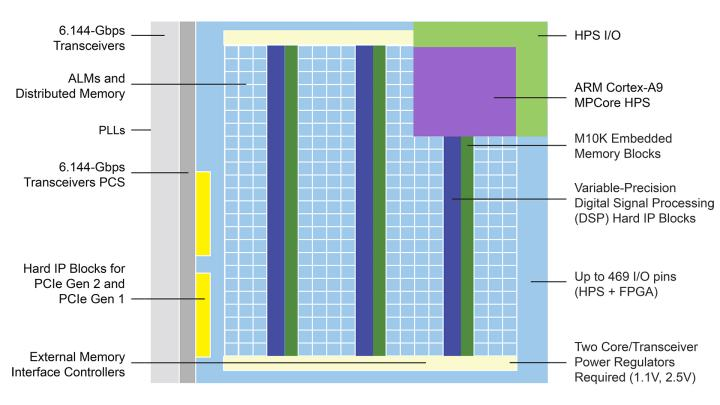
\includegraphics[width=1\linewidth]
    {../images/altera_cyclone_v_soc_architectural_downscale.jpg}
    \caption[Arquitetura da FPGA Intel Cyclone V SoC]
        {Arquitetura da \textit{FPGA Altera Cyclone V SoC} \quad Fonte: Intel
        }\label{fig:cyclone_v_arch}
\end{figure}

    \subsection{Adaptative Logic Modules}
    {}

    \begin{figure}[H]
    \centering
    \includesvg[inkscapeformat=png,width=1\linewidth]
        {../images/intel_alm_high_level.svg}
        \caption[Diagrama de blocos de um ALM]
            {Diagrama de blocos de um ALM\quad Fonte: Intel
            }\label{fig:fpga_alm}
    \end{figure}


    \subsection{Embedded Memory Blocks}
    {}

    \subsection{Hard Processor System}
    {}

    \subsection{Phase-Locked Loops}
    {}

\section{A Placa de Desenvolvimento DE1-SoC}



% \chapter{Implementação}\label{cap_implementacao}

%\resumodocapitulo{Resumo opcional}

\section{Caminho de Dados}
{
    O caminho de dados projetado para a implementação da microarquitetura
    uniciclo é apresentado na Figura~\ref{fig:datapath}.
}

\begin{figure}[H]
\centering
    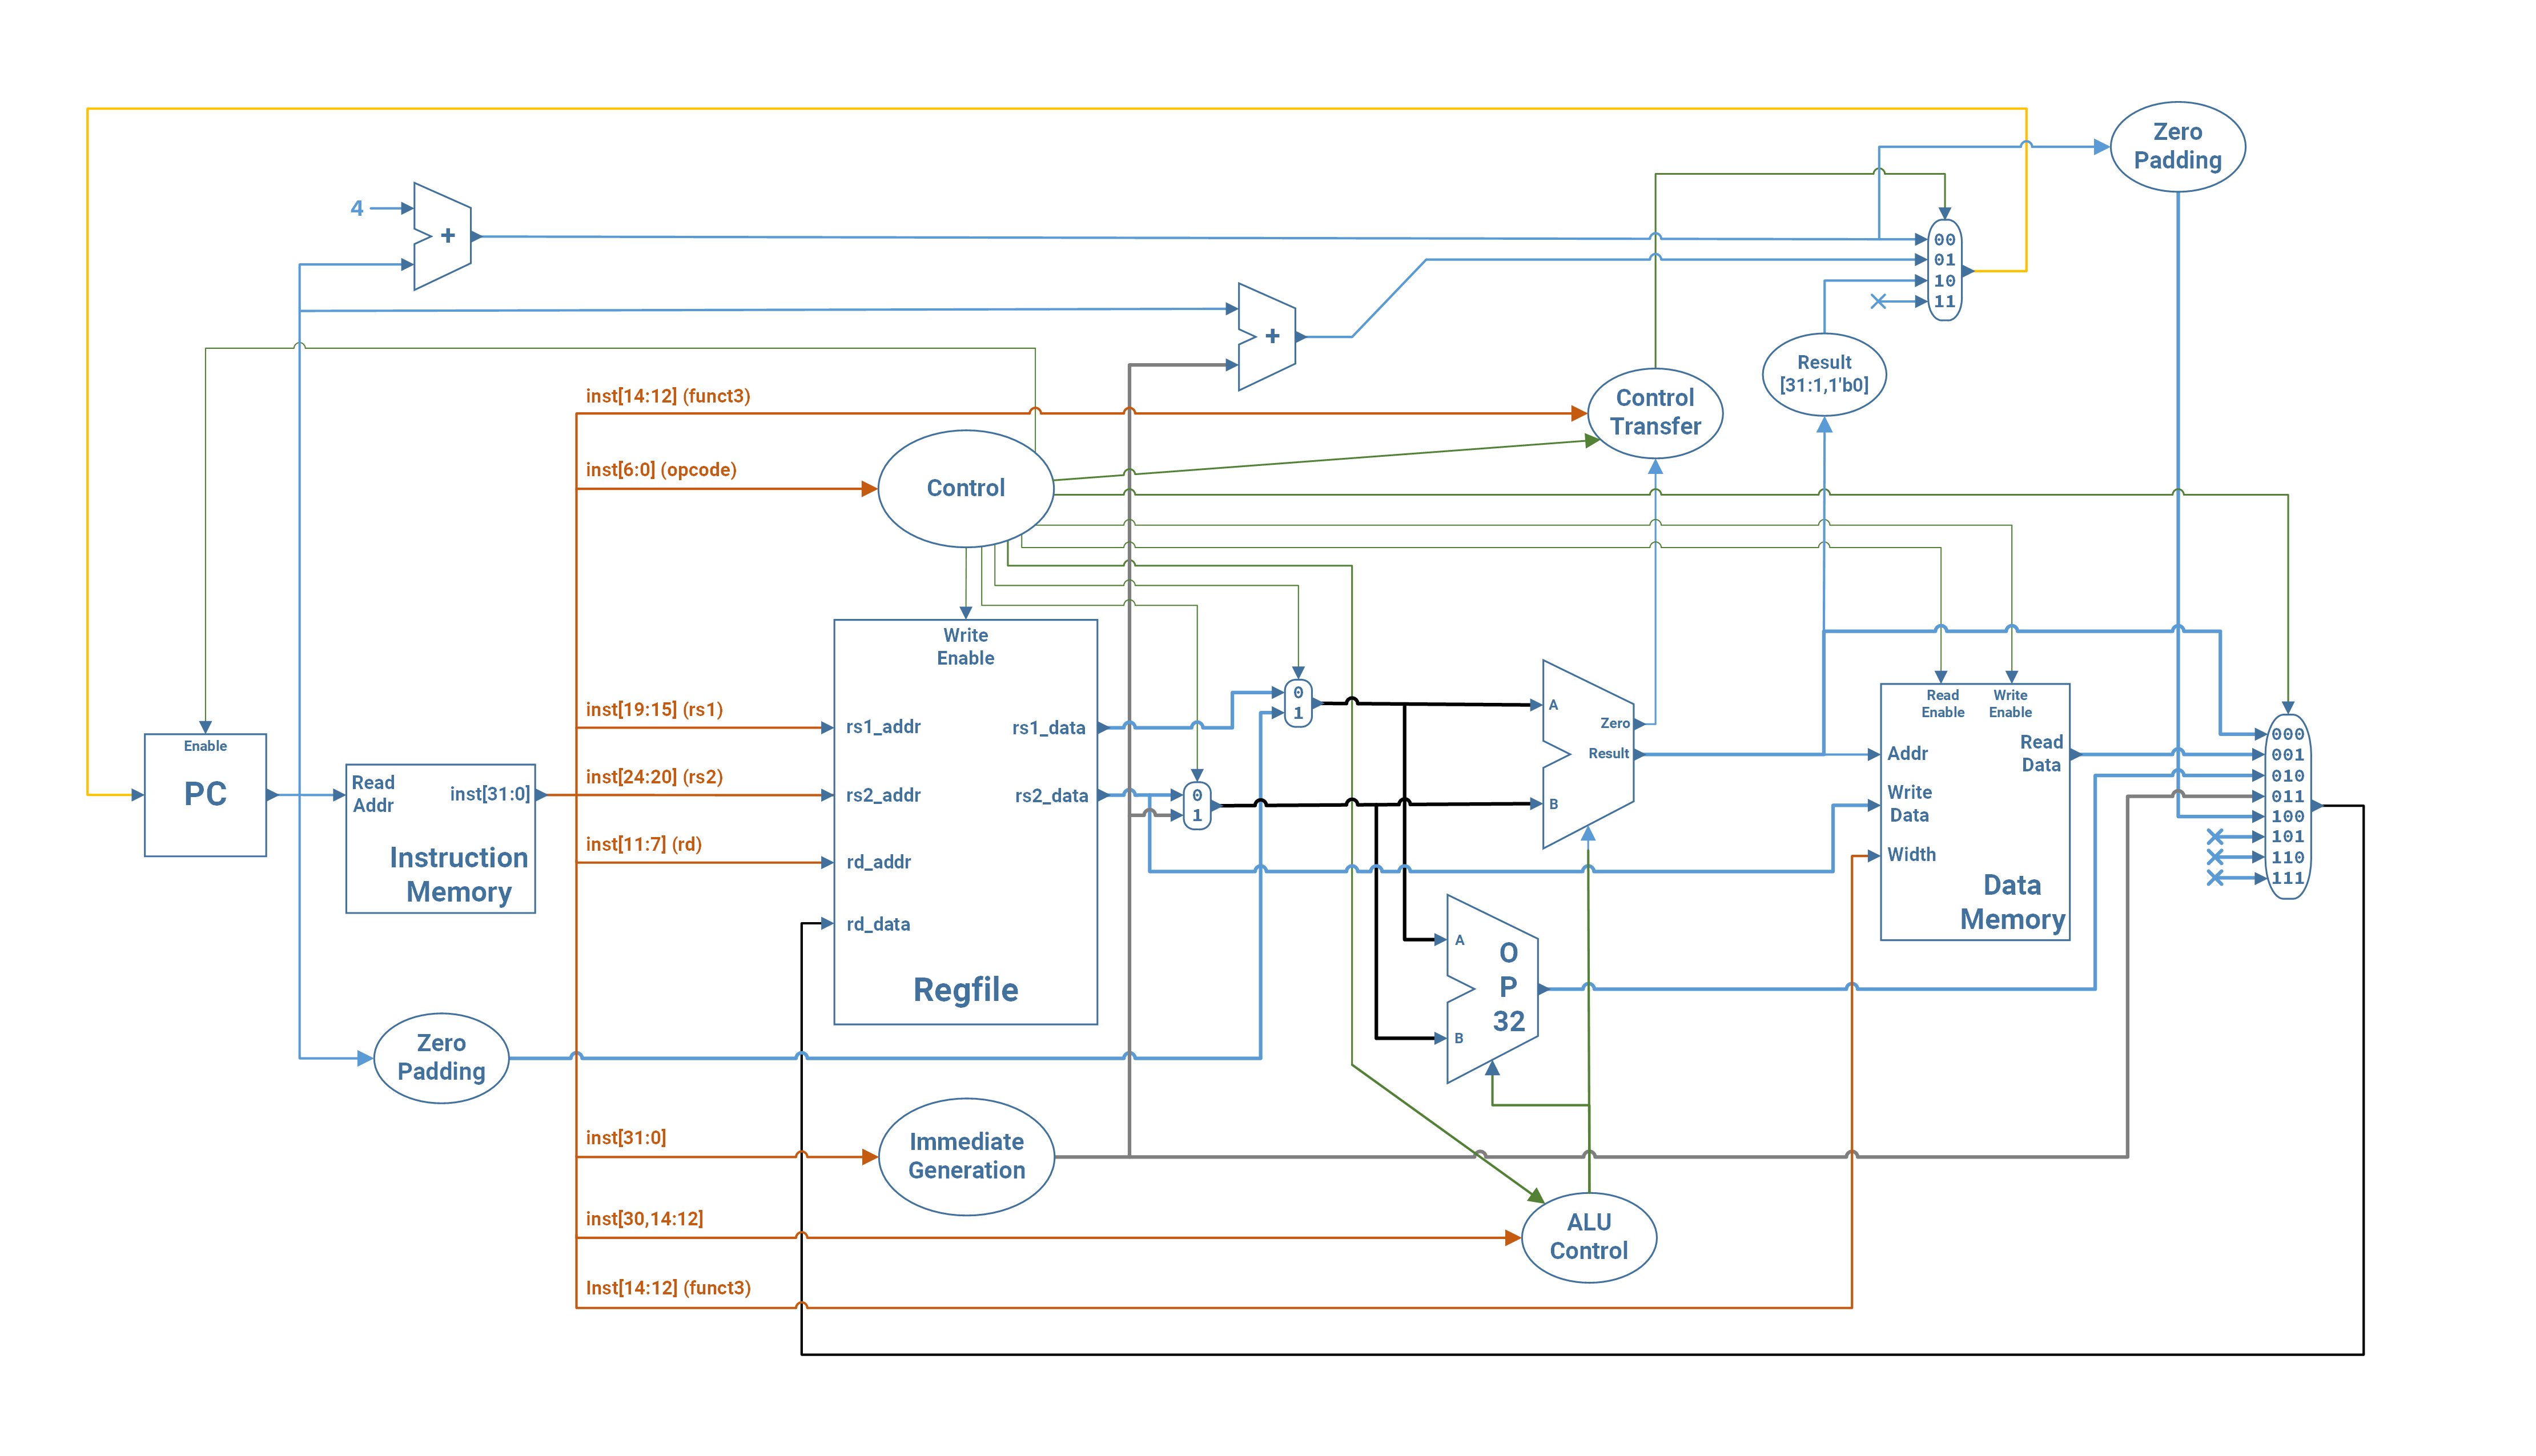
\includegraphics[width=1\linewidth]{../images/singlecycle.png}
    \caption{Caminho de Dados implementado para o
                módulo I}\label{fig:datapath}
\end{figure}

{
    O \textit{datapath} possui um banco de 32 registradores de uso geral
    de 64 bits cada. A memória possui arquitetura Harvard, sendo a memória
    de instruções (\textit{text}) \textit{read-only} e a memória de dados
    (\textit{data}) \textit{read-write}.
    São implementadas 49 instruções, sendo elas:
}

\begin{itemize}[leftmargin=20mm]
    \item {LUI:\@ Load Upper Intermediate;}
    \item {AUIPC:\@ Add Upper Intermediate to Program Counter;}
    \item {JAL:\@ Jump And Link;}
    \item {JALR:\@ Jump And Link Register;}
    \item {BEQ:\@ Branch if EQual;}
    \item {BNE:\@ Branch if Not Equal;}
    \item {BLT:\@ Branch if Less Than;}
    \item {BGE:\@ Branch if Greater or Equal;}
    \item {BLTU:\@ Branch if Less Than Unsigned;}
    \item {BGEU:\@ Branch if Greater or Equal Unsigned;}
    \item {LB:\@ Load Byte;}
    \item {LH:\@ Load Halfword;}
    \item {LW:\@ Load Word;}
    \item {LBU:\@ Load Byte Unsigned;}
    \item {LHU:\@ Load Halfword Unsigned;}
    \item {SB:\@ Store Byte;}
    \item {SH:\@ Store Halfword;}
    \item {SW:\@ Store Word;}
    \item {ADDI:\@ ADD Immediate;}
    \item {SLTI:\@ Set on Less Than;}
    \item {SLTIU:\@ Set on Less Than Unsigned;}
    \item {XORI:\@ XOR Immediate;}
    \item {ORI:\@ OR Immediate;}
    \item {ANDI:\@ AND Immediate;}
    \item {SLLI:\@ Shift Left Logical Immedate;}
    \item {SRLI:\@ Shift Right Logical Immediate;}
    \item {SRAI:\@ Shift Right Arithmetic Immediate;}
    \item {ADD:\@ ADD;}
    \item {SUB:\@ SUB;}
    \item {SLL:\@ Shift Left Logical;}
    \item {SLT:\@ Set on Less Than;}
    \item {SLTU:\@ Set on Less Than Unsigned;}
    \item {XOR:\@ XOR;}
    \item {SRL:\@ Shift Right Logical;}
    \item {SRA:\@ Shift Right Arithmetic;}
    \item {OR:\@ OR;}
    \item {AND:\@ AND;}
    \item {LWU:\@ Load Word Unsigned;}
    \item {LD:\@ Load Double;}
    \item {SD:\@ Store Double;}
    \item {ADDIW:\@ ADD Immediate Word-size;}
    \item {SLLIW:\@ Shift Left Logical Immedate Word-size;}
    \item {SRLIW:\@ Shift Right Logical Immediate Word-size;}
    \item {SRAIW:\@ Shift Right Arithmetic Immediate Word-size;}
    \item {ADDW:\@ ADD Word-size;}
    \item {SUBW:\@ SUB Word-size;}
    \item {SLLW:\@ Shift Left Logical Word-size;}
    \item {SRLW:\@ Shift Right Logical Word-size;}
    \item {SRAW:\@ Shift Right Arithmetic Word-size;}
\end{itemize}

{
    Para que o processador seja completamente compatível com a
    especificação da \textit{ISA}, falta implementar tratamentos de
    exceções, interrupções e \textit{traps}, Registradores \textit{CSR},
    instruções de chamada ao ambiente (ECALL/EBREAK), instruções de
    \textit{fencing} de memória, suporte ao acesso desalinhado à memória
    de dados e pilha de endereço de retorno (RAS).
}


\chapter{Resultados}\label{cap_resultados}

%\resumodocapitulo{Resumo opcional}

\chapter{Conclusões}\label{cap_conclusoes}

\section{Perspectivas Futuras}



% % Bibliografia
\renewcommand{\bibname}{REFERÊNCIAS BIBLIOGRÁFICAS}
\addcontentsline{toc}{chapter}{REFERÊNCIAS BIBLIOGRÁFICAS}


\bibliographystyle{abnt-num}
\bibliography{relatorio.bib}

% Anexos
\anexos{}
\makeatletter
\renewcommand{\@makechapterhead}[1]{
  { \parindent\z@ \raggedleft\setfontarial\bfseries
    \LARGE \thechapter. \space\space \uppercase{#1}\par \vskip 40\p@
  }
}
\makeatother

% Anexo I: Descrição do CD

\chapter{Descrição do conteúdo do CD}

\label{AnCD}

Descrever CD.


\refstepcounter{noAnexo}

% Anexo II: Programas Utilizados

\chapter{Programas utilizados}

Quais programas foram utilizados?


\refstepcounter{noAnexo}

\end{document}
